% Straight up stealing preamble from Eli Holmes 
%%%%%%%%%%%%%%%%%%%%%%%%%%%%%%%%%%%%%%START PREAMBLE THAT IS THE SAME FOR ALL EXAMPLES
\documentclass{article}

%Required: You must have these
\usepackage{Sweave}
\usepackage{graphicx}
\usepackage{tabularx}
\usepackage{hyperref}
\usepackage{natbib}
\usepackage{pdflscape}
\usepackage{array}
\usepackage{gensymb}
%\usepackage[backend=bibtex]{biblatex}
%Strongly recommended
 %put your figures in one place
 
%you'll want these for pretty captioning
\usepackage[small]{caption}

\setkeys{Gin}{width=0.8\textwidth} %make the figs 50 perc textwidth
\setlength{\captionmargin}{30pt}
\setlength{\abovecaptionskip}{0pt}
\setlength{\belowcaptionskip}{10pt}
% manual for caption http://www.dd.chalmers.se/latex/Docs/PDF/caption.pdf

%Optional: I like to muck with my margins and spacing in ways that LaTeX frowns on
%Here's how to do that
 \topmargin -2cm     
 \oddsidemargin -0.04cm   
 \evensidemargin -0.04cm  % same as oddsidemargin but for left-hand pages
 \textwidth 16.59cm
 \textheight 22.94cm 
 %\pagestyle{empty}       % Uncomment if don't want page numbers
 \parskip 7.2pt           % sets spacing between paragraphs
 %\renewcommand{\baselinestretch}{1.5} 	% Uncomment for 1.5 spacing between lines
\parindent 0pt% sets leading space for paragraphs
\usepackage{setspace}
%\doublespacing

%Optional: I like fancy headers
\usepackage{fancyhdr}
\pagestyle{fancy}
\fancyhead[LO]{Do early phenological events constrain later phenology?}
\fancyhead[RO]{2017}
 
%%%%%%%%%%%%%%%%%%%%%%%%%%%%%%%%%%%%%%END PREAMBLE THAT IS THE SAME FOR ALL EXAMPLES

%Start of the document
\begin{document}

% \SweaveOpts{concordance=TRUE}
\bibliographystyle{/Users/aileneettinger/citations/Bibtex/styles/amnat.bst}
\title{Do early phenological events constrain later phenology?} 
\author{A.K. Ettinger, S. Gee, and E.M. Wolkovich}
%\date{\today}
\maketitle  %put the fancy title on
%\tableofcontents      %add a table of contents
%\clearpage
%%%%%%%%%%%%%%%%%%%%%%%%%%%%%%%%%%%%%%%%%%%%%%%%%%%

%We plan to submit this paper as a ``brief communication' at American Journal of Botany (``short (3000-5000 word) research articles reporting exciting, significant new findings. They include no more than 4 figures and tables, combined. Manuscripts, and their abstracts, should be organized as described for Research articles.") or a ``rapid report" at New Phytologist.

\section*{Abstract}
\subsection*{Premise of the study}
We test the extent to which previous plant phenological stages constrain later ones, throughout a growing season and across 25 angiosperm tree species. 
\subsection*{Methods}
\subsection*{Key results}
\subsection*{Conclusions}
\section* {Key words}
plant phenology, climate change, bud-burst, leaf-out, angiosperm, tree
\section* {Introduction}
Plant phenology, the timing of life-events such as leaf-out and flowering, is a critical trait that affects individual fitness, population abundance, agricultural and natural productivity, and global climate, through its role in carbon sequestration \citep{miller-rushing2008,primack2009a,willis2010,miller-rushing2010}. In many plant species, phenology is controlled at least partially by temperature. As such, phenology has been affected by anthropogenic climate change, and is expected to be altered further by future climate change\citep{parmesan2006}. Because of its important role in many ecosystem services, planning and preparing for climate change impacts will benefit from improved understanding and forecasting of phenology.
\par Despite the observation that plant phenology generally shifts earlier with warmer temperatures, dramatic variation exists in phenological responses to climate. Different plant species vary widely in the timing of leaf out and other phenological processes, even when exposed to the same environmental conditions \citep{lechowicz1984,primack2009c}. For example, spring leaf out can span weeks among coexisting tree species \citep{lechowicz1984}. The drivers of these variations are poorly understood, even though phenology has been long-observed \citep{wolkovich2014}.
\par One important feature of plant phenology is that events are sequential: leaf bud-burst comes before leaf-out and flowering comes before fruiting. This ordering may constrain phenological events but the extent of constraints between phenological events is poorly understood, because few studies have integrated across events. Here, we examine the extent to which previous phenological events constrain later events. Specifically, we test two hypotheses:
\begin{itemize}
\item Hypothesis 1: Previous phenological events constrain later events; e.g., late-fruiting species set fruit late in the season because they leaf-out late  (Figure \ref{fig:hyp}).
\item Hypothesis 2: Inter-phenophase time  constrains phenology; e.g., late-fruiting species set fruit late in the season because they require longer development time (Figure \ref{fig:hyp}).
\end{itemize}

\section* {Materials and Methods}
\subsection*{Study site and focal species}
This study was conducted at the Arnold Arboretum of Harvard University, a 281-acre park in Boston, Massachusetts, established in 1872. It contains a living collection of 3,825 woody plant taxa, which are native to North America, Europe, and Asia. Arboreta are great resources for phenological studies across many species \citep{primack2009a}, particularly in temperate areas, since they may contain a higher diversity of tree species growing in one location than nearby natural areas. In addition, there is often high variation in phenology in the species planted in arboreta, for public enjoyment. For this study, we selected 25 focal angiosperm species that varied in their flowering times (Table 1). We selected up to five individuals of each species for the study, yielding a total of 118 individuals.

\subsection*{Phenology data collection}
Phenology was quantified following the National Phenology Network (NPN) protocols \citep{denny2014}. The budburst phase is characterized by the green leaf tips visible at the tips of buds. Leaf out phase is characterized by visible fully unfolded leaves and petioles that have completely emerged from the buds. Leaf senescence phase is characterized by leaves changing from green to fall colors. Flowering phase is when open flowers are visible. Fruiting phase is when developing fruit are visible. 
\par We visited each individual once every 6-10 days throughout the growing season. Phenology observations in the spring began on April 6, 2015, and fall phenology observations ended on December 2, 2015.
From the phenology data, we extracted the day of the year (DOY) of the first observed occurrence of a given phenological phase. Bud-burst DOY was defined as the first day when three or more leaf buds were seen bursting. Leaf out DOY was defined as the first day when 5\% or more of the individual was leafing out. Flowering DOY was defined as the first day when 5\% or more of the flower buds were open. Fruiting DOY was defined as the first day when three or more developing fruits were observed on the individual. Leaf senescence DOY was defined as the first day when 5\% or more of the individual showed fall colors. (These definitions follow NPN protocols.)
\subsection*{Statistical analyses}
To understand the extent to which previous phenological events constrain later events (Hypothesis 1, Figure \ref{fig:hyp}), we fit linear models with each phenological stage that we observed (except budburst, the earliest stage we quantified) as the response variable (i.e. species-level mean day of year of leaf-out, flowering, fruiting, or senescence).  We fit 10 different models, each with one of the previous phenological stages as the explanatory variable. 
All analyses were conducted in R version 3.2.4 \citep{rcoreteam2016}.

\section* {Results}
\par Bud-burst occurred over 32 days in the spring, and leaf-out occurred over 30 days, across all focal species \ref{fig:focsp}. Flowering phenology occurred over a longer period than bud-burst and leaf-out, spanning 111 days from late April to September \ref{fig:focsp}. Fruiting spanned 183 days, and leaf senescence occurred over 56 days\ref{fig:focsp}. Most individuals spent the majority of the growing season in the reproductive phenological phases (i.e. flowering and fruit development) \ref{fig:focsp}.%I took these numbers from Sally's thesis, but i'm actually not sure how she got them...they don't seem to match the average numbers that appear in ref{fig:focsp}
\par We found strong correlations between late versus early phenology stages in many cases (Figures \ref{fig:focsp}, \ref{fig:latevearly}), suggesting  Our that earlier phenological stages constrain later ones. The strongest correlations occurred between adjacent stages (i.e. those along the diagonal in Figure \ref{fig:latevearly}, such as leaf-out and budburst, fruiting and flowering). Senescence was the only phenological stage not well-correlated with an earlier phanological stage.
\par We also observed strong correlations between phenology and interphenophase duration for budburst and for reproductive stages (flowering and fruiting time, Figure \ref{fig:inter}). Reproductive phenology appears to be constrained by both earlier inter-phenophase times (e.g. time between flowering and budburst, time between fruiting and flowering) and later interphase times (e.g. time between senescence and flowering). Bud-burst day of year, which was the earliest phenophase we observed in the growing season, was most strongly related to inter-phenophase time between leaf-out and budburst. For other growth phenophases (leaf-out, senescence), inter-phenophase time was not a strong predictor of phenology (Figure \ref{fig:inter}). 

\section* {Discussion}

Leaf-out, flowering, and fruiting support hypothesis 1: their timing appears to be constrained by earlier phenological stages.  
Add references/studies that may explain physiology behind this, or have observed something that concurs with this? These constraints in phenological events likely create correlations among other traits. For example, frost tolerance may critically control bud-burst date, which in turn affects leaf-out, flowering, and fruiting dates, and thus could create a correlation between frost tolerance and fruit size (think about this example and look at lit to choose best example...).
\par Flowering and fruiting also support hypothesis 2: their timing appears to be constrained by inter-phenophase time. Fruiting takes about 0-20 days for most species. Add references/studies that may explain physiology behind this, or have observed something that concurs with this?

\par Our two hypotheses are not mutually exclusive. Constraints on phenology may be species-specific. 
\par Bud-burst and inter-phenophase time relationship suggests that earlier budburst does not always result in earlier leaf-out (although many species did that burst their buds early did also leaf out early, Figure \ref{fig:latevearly}). For some species, earlier budburst is simply associated with longer time between budburst and leaf-out (Figure \ref{fig:inter}). From our data, it is not clear if this pattern is due to variation in species' physiology and drivers of phenology, or to weather patterns. For example, many species leafed out after day 130, despite budburst days ranging from day 110 to 130. Weather conditions during the spring of 2015 were cold and wet, with warming occurring suddenly on day XXX (just an idea- i have no idea if this is true! need to look at the data). Multi-year studies will be critical. 
\par Expect correlations could be strongest  at biggest at end of season. Geometric constraint.
\par Implications of these constraints
\section* {Conclusions}
Next steps: Encourage a phylogenetic approach, collect data across years. We observed variation at whole organism level- may want to explore at individual flower/fruit level. 

Excerpts from sally's thesis that i want to include:
Plant phenology occupies a temporal niche, and each phase is linked to phases that occur before or concurrently with it  \citep{wolkovich2014}. At the beginning of the growing season, leaf development overlaps with flowering in some species (Figure 1). Across the 25 species in this study, bud burst occurred before leaf out and both bud burst and leaf out occurred before flowering as seen by the significant positive relationships between adjacent phenological phases (Table 3). Flowering is then followed by fruiting (Figure 1; Table 3). Fruiting is then followed by leaf senescence at the end of the growing season (Figure 1; Table 3). The end of the growing season ended with leaf senescence in most species, but some species were still undergoing fruit ripening after leaf senescence (Figure 1). This demonstrates that even though phenological phases do overlap, there is generally an ordered sequence of phenological events. Any changes to one or more of these phenological phases with climate change have the potential to impact following phases  \citep{wolkovich2014b}. This suggests that effects of any functional trait on one phenological phase may indirectly affect other phenological phases as well.
In addition, it would be beneficial to extend my study over multiple years, to evaluate the extent to which the patterns I observed are consistent among years that may vary in climate, as well as biotic conditions (i.e. pollinator or pest populations). A long-term study linking phenology and other traits to performance (i.e. growth, reproduction) is required to fully understand how phenology and phenological shifts will affect plant populations in a warming world. The ability to forecast phenological shifts and their consequences with climate change will help predict how ecosystem functions will be altered with climate change.

Leaf senescence is less studied and more poorly understood, compared to spring phenological phases (Parmesan, 2006). However, it is important that future studies focus on understanding this phenological phase, since it can drive changes in growing season length (Jeong et al., 2011), and since climate change is linked to the phenomenon of later fall (Richardson et al. 2006; Jeong et al., 2011).
\section*{Acknowledgements}
We thank H. Eyster, D. Flynn, E. Forrestel, S. Golumbeanu, W. Friedman, R. Mcnellis, J. Samaha, J. Savage, and T. Savas for field and laboratory assistance and advice. We thank J. DelRosso, M. Dosmann, A. Gapinski, K. Richardson, F. Rosin, and the many other curatorial, horticultural, and research staff of the Arnold Arboretum who made this work possible. Research was supported by the Harvard College Research Program (to S.G.), the Grants-In-Aid of Undergraduate Research program of the Museum of Comparative Zoology, the Harvard University Herbaria, and the Arnold Arboretum of Harvard University (to S.G.), and the National Science Foundation (NSF DBI 14-01854 to A.E.). Any opinion, findings, and conclusions or recommendations expressed in this material are those of the authors and do not necessarily reflect the views of the National Science Foundation.

\section*{Data Accessibility}
The dataset for this study is available online at KNB (Cite). 

\section*{Author contributions} All authors conceived and designed the study and edited the manuscript; S.G. conducted the field and lab work; S.G. and A.E. analyzed the data and wrote the manuscript; E.W. edited the manuscript.

\section{Bibliography}
\bibliography{/Users/aileneettinger/citations/Bibtex/mylibrary}

\section* {Tables}

\begin{table}[p]
  \caption{\textbf{Focal species.} Twenty-five angiosperm species were selected, based on their flowering phenology. The number of individuals of each species observed at the Arnold Arboretum from spring through fall 2015 is in parentheses.}
\begin{footnotesize} 
   \begin{tabular}{| p{5.5cm} | p{5.5cm} | p{5.5cm} |}
    \hline
  \bf{Early season flowering} & \bf{Mid season flowering} & \bf{Late season flowering} \\ \hline
    \textit{Aesculus flava} (5) & \textit{Carya glabra} (5) & \textit{Catalpa speciosa} (5) \\ 
    \textit{Betula alleghaniensis} (5) & \textit{Carya ovata} (5) & \textit{Kalopanax septemlobus} (3) \\ 
    \textit{Betula nigra} (5) & \textit{Crataegus crus-galli} (5) & \textit{Styphnolobium japonicum} (5) \\ 
\textit{Gleditsia triancanthos} (5) & \textit{Fagus engleriana} (4) & \textit{Tilia americana} (5) \\ 
\textit{Liriodendron tulipifera} (5) & \textit{Fagus grandifolia} (5) & \textit{Tilia japonica} (5) \\ 
\textit{Phellodendron amurense} var. \textit{lavallei} (4) & \textit{Fraxinus chinensis} (5) &\\ \textit{Populus deltoids} ssp. \textit{deltoids} (5) & \textit{Liquidambar styraciflua} (5) & \\ 
\textit{Pyrus calleryana} var. \textit{dimorphophylla} (3) & \textit{Platanus occidentalis} (5) & \\ 
\textit{Pyrus ussuriensis} var. \textit{hondoensis} (5) & \textit{Quercus glandulifera} (4) & \\ \textit{Quercus alba} (5) & \textit{Quercus rubra} (5) &  \\ \hline
     \end{tabular}    
\end{footnotesize} 
    \end{table}
\clearpage

\section* {Figures}
\begin{figure}[p]
  \centering
  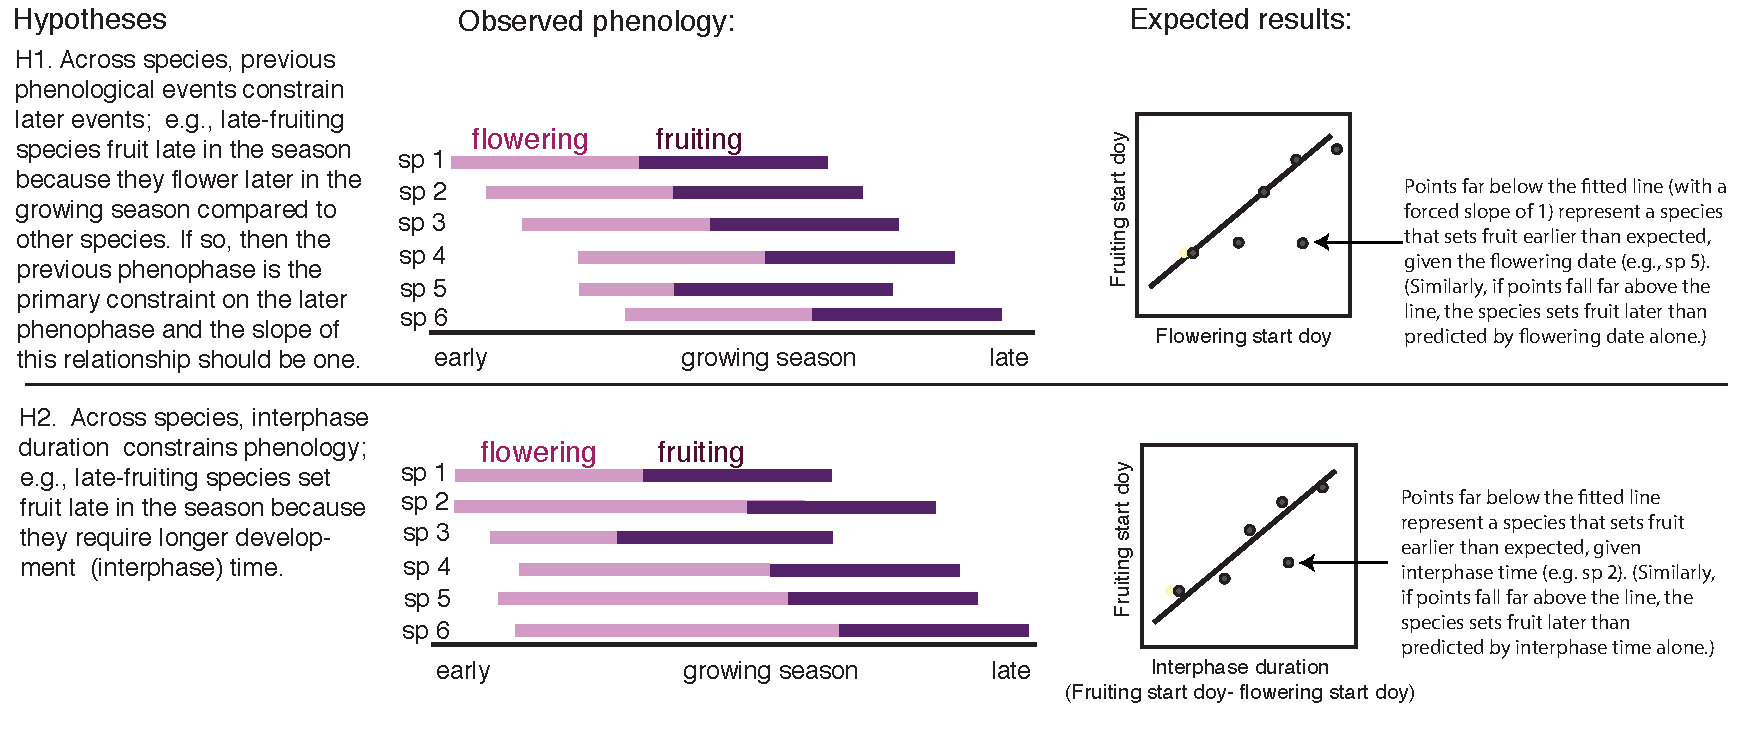
\includegraphics{../analyses/figures/hypotheses3.pdf} 
  \caption{\textbf{Hypotheses.} We show flowering and fruiting as examples of consecutive phenological events. We expected the same patterns for other consecutive events,such as leaf bud-burst and leaf-out. Inter-phenophase duration is the time between phenological events, e.g., the number of days between the start of flowering and the start of fruiting.} 
 \label{fig:hyp}
\end{figure}
 
\begin{figure}[h]
  \centering
  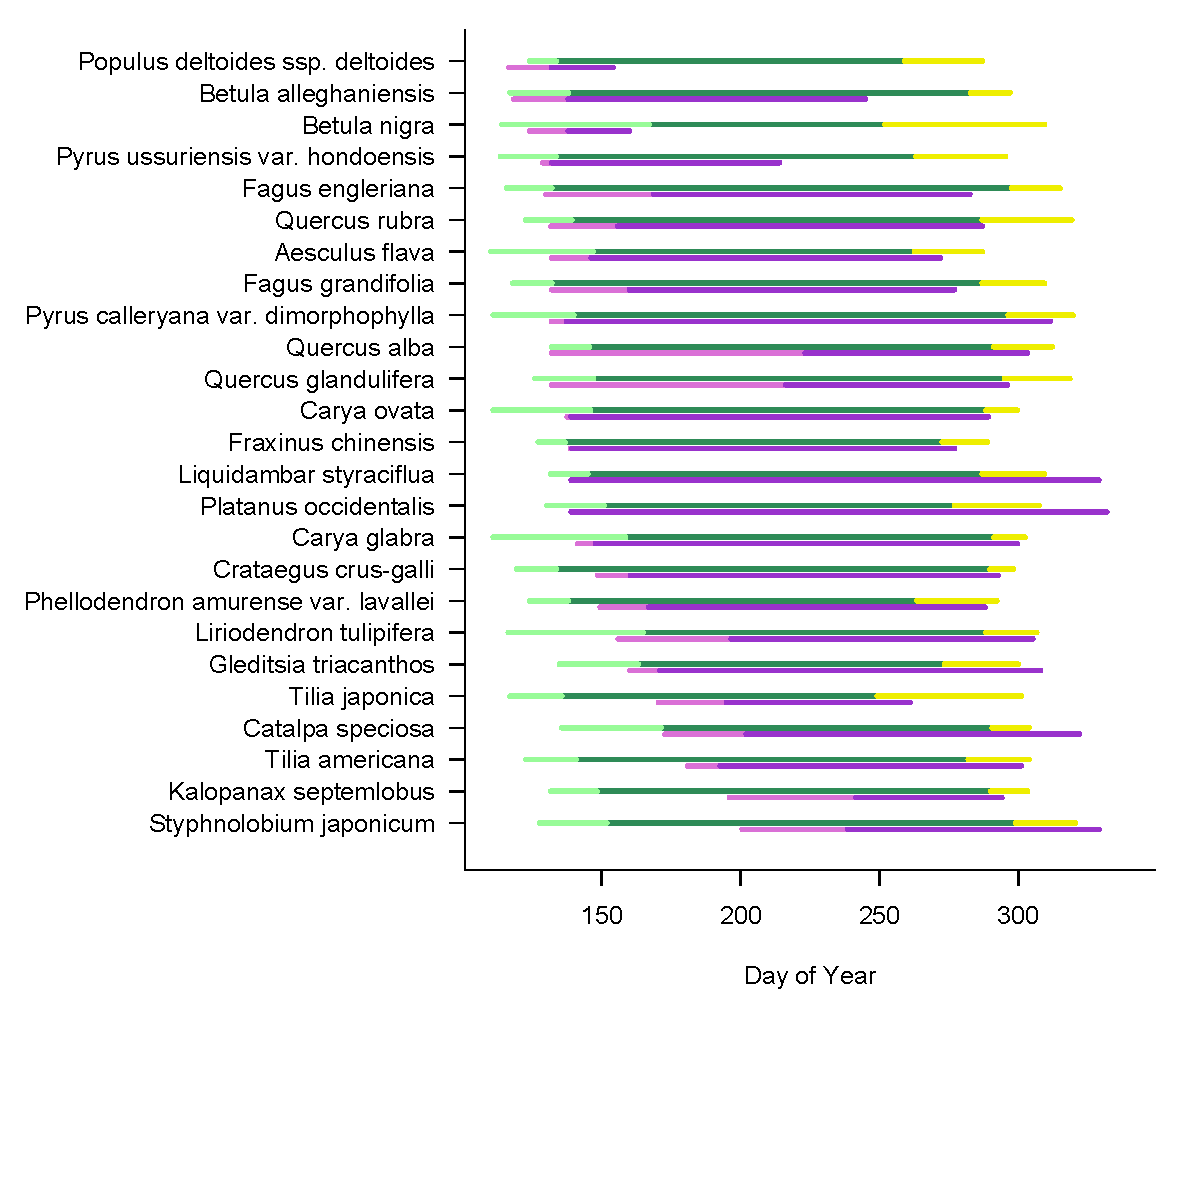
\includegraphics{../analyses/figures/grosea_repsort.pdf}
  \caption{\textbf{Focal species' phenology during the 2015 growing season, sorted by their mean first-flower dates.} For growth phenology, light green represents the bud-burst phase (from its mean start day-of-year to the mean start day-of-year for leaf-out, across all individuals within a species), dark green represents full leaf-out (from the mean day-of-year when fully-expanded leaves were first observed through the start of senescence), and yellow represents the senescence phase (from the mean day-of-year when leaves first began changing color through the mean day-of-year when more than 95 percent of leaves on the tree had changed color). For reproductive phenology, light purple represents the flowering phase (from the mean day-of-year when flowers first appeared to the mean day-of-year when fruits first appeared, across all individuals within a species) and dark purple represents the fruiting phase (from the mean day-of-year when fruits first appeared to the mean day-of-year when more than 95 percent of fruits were first observed as ripe).}
  \label{fig:focsp}
\end{figure}
  
  \begin{figure}[h]
  \centering
  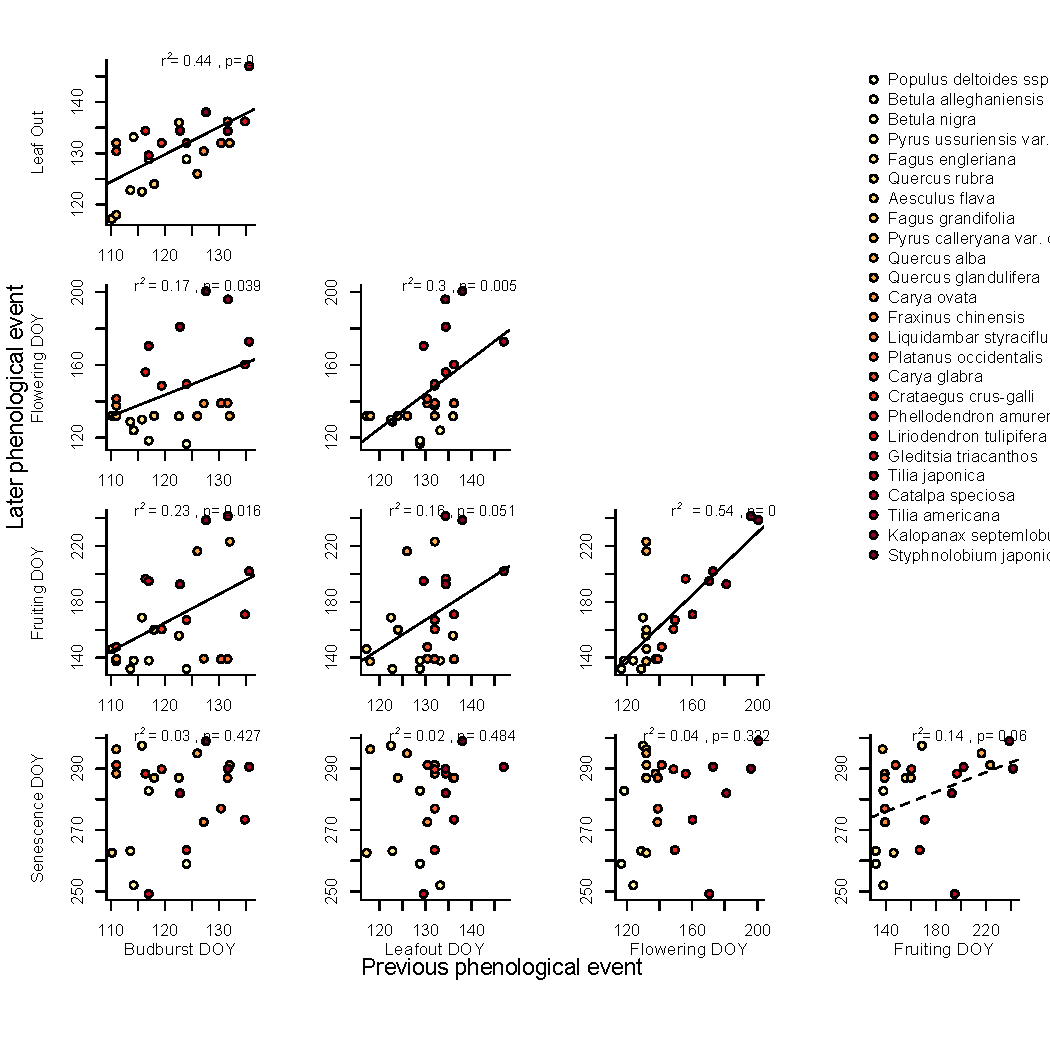
\includegraphics{../analyses/figures/latevearly_rp_col_legend_YOR.pdf}
  
  \caption{\textbf{Relationships among phenological stages across the 25 focal species.} Linear models were fit with the species-level mean day of year of the later phenological stages as the response variable, and mean day of year of earlier stage as the explanatory variable. R\textsuperscript{2} and \textit{p}-value for each model are shown, with solid lines representing model fit when \textit{p}<0.05 and dashed lines representing model fit when 0.05<\textit{p}<0.10. Full model statistics are summarized in Table S1 in the Supplemental Materials. Species in the legend are ordered from early to late first flower dates, as in Figure 2.}
  \label{fig:latevearly}
\end{figure}
\begin{figure}[h]
  \centering
  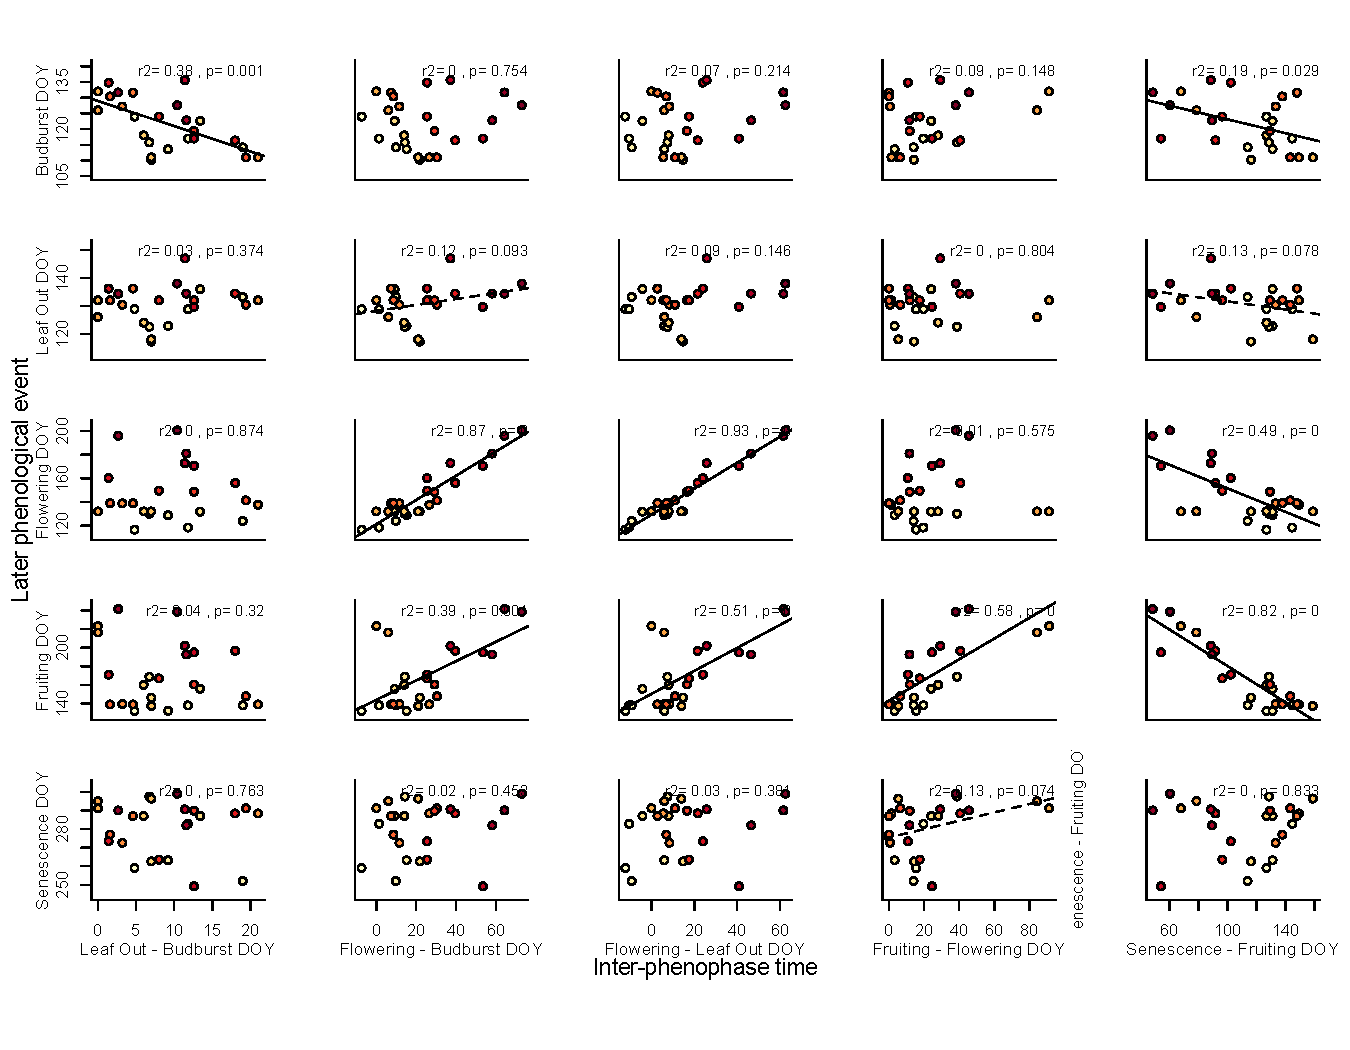
\includegraphics{../analyses/figures/adj_stagesmegaplot_col_YOR.pdf}
  \caption{\textbf{Relationships among phenological stages and inter-phenophase duration across the 25 focal species.} Inter-phenophase duration is the time between the start of the earlier phenological event and the start of the later phenological event, e.g., the number of days between the species' mean start of flowering and its mean start of fruiting. Linear models were fit with the species-level mean day of year of the later phenological stages as the response variable, and interphenophase duration as the explanatory variable. R\textsuperscript{2} and \textit{p}-value for each model are shown, with solid lines representing model fit when \textit{p}<0.05 and dashed lines representing model fit when 0.05<\textit{p}<0.10. Full model statistics are summarized in Table S1 in the Supplemental Materials. Species are color-coded as in Figure 3.}
  \label{fig:inter}
   \end{figure}


%%%%%%%%%%%%%%%%%%%%%%%%%%%%%%%%%%%%%%%%
\end{document}
%%%%%%%%%%%%%%%%%%%%%%%%%%%%%%%%%%%%%%%%
